\documentclass[11pt]{article}
\usepackage{newtxtext,newtxmath}
\usepackage{amsmath}%,amssymb}
\usepackage{geometry}
\usepackage{graphicx}
\usepackage{setspace}

% Packages for Polish language and character encoding
\usepackage[utf8]{inputenc} % For UTF-8 encoding
\usepackage[T1]{fontenc} % For proper hyphenation and accents in Polish

\thispagestyle{empty}

\geometry{a4paper, left=15mm, right=15mm, top=20mm, bottom=10mm} % please to not change the margins

\usepackage[
   colorlinks,
   linkcolor=blue,
   urlcolor=blue,
   citecolor=blue,
   ]{hyperref}

\newcommand{\abstracttitle}[1]{
\setstretch{1.15}    %increase the space between the two lines of the title
 \begin{center}{\Large {\bf #1}}\end{center}
\setstretch{1.0}
}

\newcommand{\authors}[1]{
 \begin{center}{\bf #1} \end{center}
 \setstretch{1.0}
}

\newcommand{\addresses}[1]{
\setstretch{0.95}
 \begin{center}{\small #1} \end{center}
\setstretch{1}
}


\renewcommand\refname{\normalsize References }

\begin{document}

\abstracttitle{Closing the literature--simulation loop: an untiring, citation-grounded agent for catalyst discovery}
\authors{
\underline{Reto Stamm $^{1,~\dag}$}
}

\addresses{%
$^{1}$MACATAMO Group, University of Limerick, Limerick V94 T9PX, Ireland \\
\dag corresponding author's email: \href{mailto:reto@retostamm.com}{reto@retostamm.com}
}

Pr\'ecis~\cite{Stamm2026precis} is an open-source agentic research system
built as an \emph{untiring collaborator}: it never sleeps, works from real
feedback, and lets no claim stand without a precise citation --- a specific
paragraph in a real publication that supports it, so hallucination is
designed out rather than apologized for. Papers arrive automatically from
open-access sources and continuous citation-graph exploration; the corpus
currently holds over 22{,}000 fully ingested papers (33{,}000 tracked),
broken into roughly 3~million searchable chunks. Precomputed keywords,
summaries, and a clustered dynamic table of contents let language-model
agents locate very specific claims token-efficiently instead of reading
whole papers, and tasks can park themselves until a paper is ingested or a
human answers, then resume on their own.

Discovery runs as a perpetual \emph{literature--simulation loop}. A
discovery agent owns all chemistry and holds one proposal in flight; each
candidate is priced by a progressive-fidelity simulation ladder --- a
relax-only thermodynamic screen, then climbing-image nudged-elastic-band
barriers~\cite{Henkelman2000} under machine-learned interatomic potentials
(MACE~\cite{Batatia2022}, CHGNet~\cite{Deng2023}), then a verify tier ---
under capped budgets, and results rank on a Pareto frontier over the
campaign's objective axes (barrier, material cost, stability). The
literature sits \emph{inside} the loop, not beside it: every conjecture is
minted as a typed hypothesis finding, and between compute steps the corpus
accumulates cited evidence for and against it, so the next proposal is
informed by what the field has already measured. A refuted hypothesis
converts into a negative ruling --- cited, searchable, and excluded from
re-proposal by default --- so the loop cannot re-spend compute on ideas the
literature or its own simulations have already killed.

The loop is also honest about its own measurements. Untrusted results ---
unconverged barrier searches, detached adsorbates, symmetry-equivalent
candidates whose barriers disagree --- can never rank or graduate, but stay
visible as provisional bands, so the agent is never blind to what it has
computed. The governing design principle is to substitute thinking for
compute: one hour at the library is worth a month in the simulator, so work
runs as tight idea--probe--evaluate cycles in which every simulation is
argued with the literature before it is bought and interpreted against it
afterwards. We demonstrate the loop on NO\,$\to$\,NH$_3$ over Pd-based
catalysts (Figure~\ref{fig:Figure}).

    \begin{figure}[h]
    \begin{center}
        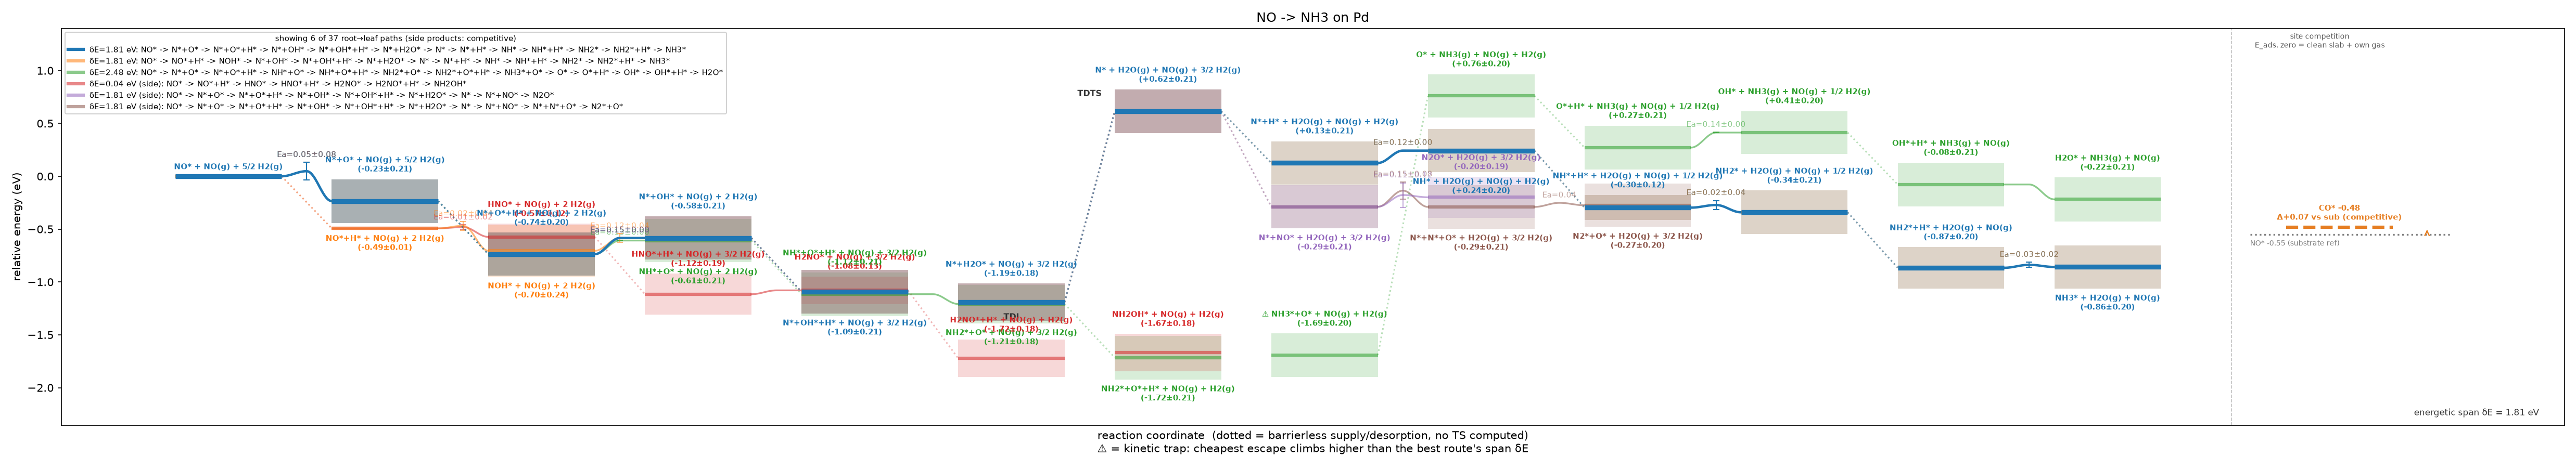
\includegraphics[width=\textwidth]{images/Figure.png}
        \caption{\label{fig:Figure}
        Reaction energy profile for NO\,$\to$\,NH$_3$ on Pd from the loop's
        simulation tier (demonstration potential): span-ranked competing
        routes at full gas composition, transition states with $E_a$ and
        uncertainty bands, kinetic-trap flags, and the CO site-competition
        panel.}
    \end{center}
    \end{figure}

\begin{thebibliography}{1}
\small
\vspace{-0.25cm}

\bibitem{Stamm2026precis} R. Stamm, {\em Pr\'ecis},
\url{https://github.com/retospect/precis-mcp} (2026).
\vspace{-0.25cm}
\bibitem{Henkelman2000} G. Henkelman, B. P. Uberuaga, and H. J\'onsson, {\em J. Chem. Phys.} {{\bf 113}, 9901 (2000).}
\vspace{-0.25cm}
\bibitem{Batatia2022} I. Batatia, D. P. Kov\'acs, G. N. C. Simm, C. Ortner, and G. Cs\'anyi, {\em Adv. Neural Inf. Process. Syst.} {{\bf 35}, 11423 (2022).}
\vspace{-0.25cm}
\bibitem{Deng2023} B. Deng {\em et al.}, {\em Nat. Mach. Intell.} {{\bf 5}, 1031 (2023).}

\end{thebibliography}

\end{document}
